\documentclass[aspectratio=169]{beamer}
\usepackage[T1]{fontenc}
\usepackage[utf8]{inputenc}

% packages
\usepackage{latexsym,amsmath,amssymb,xcolor,multicol,booktabs}
\usepackage{graphicx,listings,stackengine}
\usepackage{lipsum}
\usepackage{tikz}
\usetikzlibrary{arrows.meta,positioning,calc}

\author[Your Name]{Your Name}
\title[Short Title]{Your Presentation Title}
\subtitle{Your Subtitle}
\institute[NTNU]{Your Department, NTNU}
\date{\today}
\usepackage{NTNU}

% code listing style
\definecolor{deepblue}{rgb}{0,0,0.5}
\definecolor{deepred}{rgb}{0.6,0,0}
\definecolor{deepgreen}{rgb}{0,0.5,0}
\definecolor{halfgray}{gray}{0.55}

\lstset{
    basicstyle=\ttfamily\small,
    keywordstyle=\bfseries\color{deepblue},
    emphstyle=\ttfamily\color{deepred},
    stringstyle=\color{deepgreen},
    numbers=left,
    numberstyle=\small\color{halfgray},
    rulesepcolor=\color{red!20!green!20!blue!20},
    frame=shadowbox,
}

% ============================================================
% Timeline command
% ============================================================
% Usage: \timeline{current phase index (1-based)}{
%   {Start--End}{Label}/
%   {Start--End}{Label}/
%   ...
% }
\newcommand{\timeline}[2]{%
  \def\phasenumber{0}%
  \def\currentphase{#1}%
  \def\phases{#2}%
  \begin{tikzpicture}[
    >=Stealth,
    phase/.style={
      draw=ntnublue!60, fill=ntnusky, rounded corners=2pt,
      minimum height=0.6cm, text=black, font=\footnotesize,
      inner xsep=4pt, inner ysep=2pt,
    },
    current/.style={
      draw=ntnublue, fill=ntnublue!25, rounded corners=2pt,
      minimum height=0.6cm, text=black, font=\footnotesize\bfseries,
      inner xsep=4pt, inner ysep=2pt,
      line width=1.2pt,
    },
    timelabel/.style={font=\tiny\color{gray}},
  ]
  \def\ypos{0}%
  \def\idx{0}%
  \foreach \dates/\desc in \phases {%
    \pgfmathtruncatemacro{\idx}{\idx+1}%
    \xdef\idx{\idx}%
    \pgfmathsetmacro{\yval}{-(\idx-1)*0.9}%
    \ifnum\idx=\currentphase
      \node[current, anchor=west] (P\idx) at (2.8,\yval) {\desc};
      \node[timelabel, anchor=east] at (2.6,\yval) {\dates};
      \node[font=\scriptsize, text=ntnublue] at ($(P\idx.east)+(0.5,0)$) {$\blacktriangleleft$};
    \else
      \node[phase, anchor=west] (P\idx) at (2.8,\yval) {\desc};
      \node[timelabel, anchor=east] at (2.6,\yval) {\dates};
    \fi
  }%
  % draw connecting line
  \pgfmathtruncatemacro{\lastidx}{\idx}%
  \ifnum\lastidx>1
    \draw[ntnublue!40, line width=1.5pt]
      (P1.south west) +(-0.15,0) -- (P\lastidx.north west) +(-0.15,0);
  \fi
  % draw dots on the line
  \foreach \i in {1,...,\lastidx}{%
    \ifnum\i=\currentphase
      \fill[ntnublue] (P\i.west) +(-0.15,0) circle (3pt);
    \else
      \fill[ntnublue!40] (P\i.west) +(-0.15,0) circle (2.5pt);
    \fi
  }%
  \end{tikzpicture}%
}


\begin{document}

% ============================================================
% Title page
% ============================================================
\begin{frame}
    \titlepage
    \begin{figure}[htpb]
        \centering
        
\includegraphics[width=0.25\linewidth]{pic/ntnu-logo.pdf}
    \end{figure}
\end{frame}

% ============================================================
% Table of contents
% ============================================================
\begin{frame}
    \tableofcontents[sectionstyle=show,subsectionstyle=show/shaded/hide,subsubsectionstyle=show/shaded/hide]
\end{frame}


% ============================================================
\section{Background}
% ============================================================

\begin{frame}{Research Background}
    \begin{itemize}[<+-| alert@+>]
        \item Research motivation and context
        \item Key problem statement
        \item Why this matters
    \end{itemize}
\end{frame}


% ============================================================
\section{Literature Review}
% ============================================================

\subsection{Theoretical Foundations}

\begin{frame}{Theoretical Foundations}
    \begin{itemize}
        \item Foundational theory 1
        \item Foundational theory 2
        \item Research gap identified
    \end{itemize}
\end{frame}

\subsection{Empirical Evidence}

\begin{frame}{Empirical Evidence}
    \begin{itemize}
        \item Key finding from prior work 1
        \item Key finding from prior work 2
        \item Limitations of existing studies
    \end{itemize}
\end{frame}


% ============================================================
\section{Methodology}
% ============================================================

\subsection{Data}

\begin{frame}{Data Description}
    \begin{itemize}
        \item Data source and sample period
        \item Variable definitions
        \item Summary statistics
    \end{itemize}
\end{frame}

\subsection{Model}

\begin{frame}{Empirical Model}
    \begin{itemize}
        \item Model specification
        \item Identification strategy
        \item Robustness checks planned
    \end{itemize}
\end{frame}

\begin{frame}{Key Equation}
    The baseline regression:
    \begin{equation}
        Y_{i,t} = \alpha + \beta X_{i,t} + \gamma Z_{i,t} + \epsilon_{i,t}
    \end{equation}
    where $Y_{i,t}$ is the dependent variable, $X_{i,t}$ is the treatment, and $Z_{i,t}$ is a vector of controls.
\end{frame}


% ============================================================
\section{Results}
% ============================================================

\subsection{Main Results}

\begin{frame}{Main Results}
    \begin{itemize}
        \item Finding 1: description
        \item Finding 2: description
        \item Statistical significance and economic magnitude
    \end{itemize}
\end{frame}

\subsection{Robustness}

\begin{frame}{Robustness Checks}
    \begin{itemize}
        \item Alternative specifications
        \item Subsample analysis
        \item Placebo tests
    \end{itemize}
\end{frame}


% ============================================================
\section{Template Examples}
% ============================================================

\subsection{Formulas}

\begin{frame}{Inline \& Display Math}
    \lipsum[1][1-2] The model is $y = f(x) + \varepsilon$ where $\varepsilon \sim \mathcal{N}(0, \sigma^2)$.

    \vspace{0.5em}
    A single numbered equation:
    \begin{equation}
        \hat{\beta} = (X^\top X)^{-1} X^\top y
    \end{equation}
\end{frame}

\begin{frame}{Multiple Equations (align)}
    The CAPM and a multi-factor extension:
    \begin{align}
        E[R_i] - R_f &= \beta_i \bigl( E[R_m] - R_f \bigr) \label{eq:capm} \\
        R_{i,t} - R_{f,t} &= \alpha_i + \beta_i^{\text{MKT}} \text{MKT}_t
            + \beta_i^{\text{SMB}} \text{SMB}_t
            + \beta_i^{\text{HML}} \text{HML}_t
            + \epsilon_{i,t} \label{eq:ff3}
    \end{align}
    Equation~\eqref{eq:capm} is the CAPM; Equation~\eqref{eq:ff3} is the Fama--French three-factor model.
\end{frame}

\begin{frame}{Theorems \& Proofs}
    \begin{theorem}[Gauss--Markov]
        Under assumptions A1--A5, the OLS estimator $\hat{\beta}$ is the Best Linear Unbiased Estimator (BLUE).
    \end{theorem}

    \begin{proof}
        For any other linear unbiased estimator $\tilde{\beta} = Cy$,
        \[
            \text{Var}(\tilde{\beta}) - \text{Var}(\hat{\beta}) = \sigma^2 (C - (X^\top X)^{-1}X^\top)(C - (X^\top X)^{-1}X^\top)^\top \geq 0.
        \]
    \end{proof}
\end{frame}

\subsection{Tables}

\begin{frame}{Simple Table}
    \lipsum[2][1]
    \begin{table}[htpb]
        \centering
        \footnotesize
        \caption{Summary Statistics}
        \begin{tabular}{lcccc}
            \toprule
            \textbf{Variable} & \textbf{Mean} & \textbf{Std.\ Dev.} & \textbf{Min} & \textbf{Max} \\
            \midrule
            Return      & 0.082 & 0.154 & $-$0.421 & 0.563 \\
            Size        & 7.234 & 1.892 & 3.012  & 12.451 \\
            B/M Ratio   & 0.654 & 0.413 & 0.051  & 2.873  \\
            Leverage    & 0.312 & 0.187 & 0.000  & 0.891  \\
            \bottomrule
        \end{tabular}
    \end{table}
\end{frame}

\begin{frame}{Regression Table}
    \begin{table}[htpb]
        \centering
        \footnotesize
        \caption{Regression Results}
        \begin{tabular}{lccc}
            \toprule
            & \textbf{(1)} & \textbf{(2)} & \textbf{(3)} \\
            \midrule
            Treatment   & 0.045$^{***}$ & 0.038$^{**}$  & 0.041$^{***}$ \\
                        & (0.012)       & (0.015)       & (0.013)       \\
            Control 1   &               & 0.021$^{*}$   & 0.019$^{*}$   \\
                        &               & (0.011)       & (0.010)       \\
            Control 2   &               &               & $-$0.008      \\
                        &               &               & (0.007)       \\
            \midrule
            Fixed Effects & No  & Yes & Yes \\
            Observations  & 5{,}420 & 5{,}420 & 5{,}218 \\
            $R^2$         & 0.12  & 0.18  & 0.21  \\
            \bottomrule
            \multicolumn{4}{l}{\scriptsize $^{*}p<0.10$, $^{**}p<0.05$, $^{***}p<0.01$} \\
        \end{tabular}
    \end{table}
\end{frame}

\subsection{Figures}

\begin{frame}{Single Figure}
    \lipsum[3][1]
    \begin{figure}[htpb]
        \centering
        \begin{tikzpicture}[scale=0.7]
            \draw[->] (0,0) -- (7,0) node[right] {\footnotesize Time};
            \draw[->] (0,0) -- (0,4.5) node[above] {\footnotesize Return};
            \draw[ntnublue, thick] plot[smooth, tension=0.6] coordinates
                {(0.5,1.0) (1.5,1.8) (2.5,1.4) (3.5,2.5) (4.5,2.2) (5.5,3.2) (6.5,3.8)};
            \draw[red!70!black, thick, dashed] plot[smooth, tension=0.6] coordinates
                {(0.5,0.8) (1.5,1.2) (2.5,1.6) (3.5,1.9) (4.5,2.3) (5.5,2.6) (6.5,3.0)};
            \node[ntnublue, font=\scriptsize] at (6.5,4.2) {Portfolio};
            \node[red!70!black, font=\scriptsize] at (6.5,2.6) {Benchmark};
        \end{tikzpicture}
        \caption{Cumulative returns: portfolio vs.\ benchmark.}
    \end{figure}
\end{frame}

\begin{frame}{Two Figures Side by Side}
    \begin{figure}[htpb]
        \centering
        \begin{minipage}{0.48\textwidth}
            \centering
            \begin{tikzpicture}[scale=0.55]
                \draw[->] (0,0) -- (5,0) node[right] {\tiny $x$};
                \draw[->] (0,0) -- (0,4) node[above] {\tiny $f(x)$};
                \draw[ntnublue, thick, domain=0:4.5, samples=50]
                    plot (\x, {3.5*exp(-0.5*(\x-2.5)^2/0.8)});
                \node[font=\scriptsize] at (2.5,-0.5) {(a) Normal distribution};
            \end{tikzpicture}
        \end{minipage}%
        \hfill
        \begin{minipage}{0.48\textwidth}
            \centering
            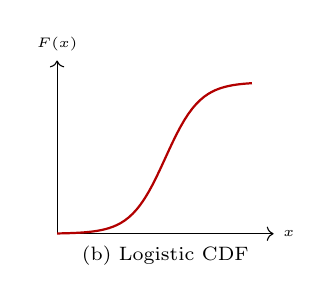
\begin{tikzpicture}[scale=0.55]
                \draw[->] (0,0) -- (5,0) node[right] {\tiny $x$};
                \draw[->] (0,0) -- (0,4) node[above] {\tiny $F(x)$};
                \draw[red!70!black, thick, domain=0:4.5, samples=50]
                    plot (\x, {3.5/(1+exp(-2.5*(\x-2.5)))});
                \node[font=\scriptsize] at (2.5,-0.5) {(b) Logistic CDF};
            \end{tikzpicture}
        \end{minipage}
        \caption{Density and cumulative distribution functions.}
    \end{figure}
\end{frame}

\begin{frame}{Figure with Text (columns)}
    \begin{columns}[T]
        \begin{column}{0.55\textwidth}
            \lipsum[4][1-3]
        \end{column}
        \begin{column}{0.42\textwidth}
            \begin{figure}[htpb]
                \centering
                \begin{tikzpicture}[scale=0.55]
                    \draw[fill=ntnusky] (0,0) rectangle (1.2,3.2);
                    \draw[fill=ntnublue!60] (1.8,0) rectangle (3.0,2.4);
                    \draw[fill=ntnublue] (3.6,0) rectangle (4.8,3.8);
                    \node[font=\tiny] at (0.6,-0.3) {Group A};
                    \node[font=\tiny] at (2.4,-0.3) {Group B};
                    \node[font=\tiny] at (4.2,-0.3) {Group C};
                    \draw[->] (0,0) -- (5.5,0);
                    \draw[->] (0,0) -- (0,4.5) node[above] {\tiny Value};
                \end{tikzpicture}
                \caption{Bar chart example.}
            \end{figure}
        \end{column}
    \end{columns}
\end{frame}

\subsection{Blocks}

\begin{frame}{Block Environments}
    \begin{block}{Definition}
        \lipsum[5][1]
    \end{block}

    \begin{alertblock}{Important}
        \lipsum[5][2]
    \end{alertblock}

    \begin{exampleblock}{Example}
        \lipsum[5][3]
    \end{exampleblock}
\end{frame}


% ============================================================
\section{Timeline}
% ============================================================

\begin{frame}{Project Timeline}
    \centering
    \timeline{3}{%
        {Sep--Dec 2025}{Literature review \& data collection}/
        {Jan--Mar 2026}{Preliminary analysis \& modeling}/
        {Apr--Jun 2026}{Main empirical analysis}/
        {Jul--Sep 2026}{Robustness \& writing}/
        {Oct--Dec 2026}{Submission \& revision}/
    }
\end{frame}

\begin{frame}{Detailed Milestones}
    \begin{table}[htpb]
        \centering
        \footnotesize
        \begin{tabular}{lll}
            \toprule
            \textbf{Phase} & \textbf{Period} & \textbf{Deliverable} \\
            \midrule
            Literature review   & Sep--Dec 2025 & Survey paper draft \\
            Data collection     & Jan--Feb 2026 & Clean dataset \\
            Model development   & Feb--Mar 2026 & Working model \\
            Empirical analysis  & Apr--Jun 2026 & Results tables \\
            Robustness          & Jul--Aug 2026 & Extended appendix \\
            Writing             & Aug--Sep 2026 & Full paper draft \\
            Submission          & Oct 2026      & Journal submission \\
            \bottomrule
        \end{tabular}
    \end{table}
\end{frame}


% ============================================================
\section{References}
% ============================================================

\begin{frame}{References}
    Cite as needed: \cite{article1}
    \begin{thebibliography}{99}
        \bibitem{article1} Author, F. and Author, S.
        \emph{Title of the Article}.
        Journal Name, 2024.
    \end{thebibliography}
\end{frame}


% ============================================================
% Thank you
% ============================================================
\begin{frame}
    \begin{center}
        {\Huge Thank You!}

        \vspace{1em}
        \normalsize
        Your Name \\
        \texttt{your.email@ntnu.no} \\
        Your Department, NTNU
    \end{center}
\end{frame}

\end{document}
